%% Transportation Research Part E submission draft (Elsevier elsarticle, author-year).
%% Overleaf compiler: pdfLaTeX. Red [TODO: ...] marks text or results that do not exist yet.
%% Draft v2 of 2026-11-02, structured after Wu et al. (2026), TR-E 209, 104742
%% (Introduction / Related work / Preliminaries / The method / Experiments / Conclusion).
%% Numbers come from outputs/ in the code repository; see the comment above each table.

\documentclass[preprint,review,12pt,authoryear]{elsarticle}
%% Journal-like layout while drafting: \documentclass[final,3p,times,authoryear]{elsarticle}

\usepackage{amssymb,amsmath,amsthm}
\usepackage{booktabs,multirow}
\usepackage{algorithm,algpseudocode}
\usepackage{graphicx,xcolor}
\usepackage{tikz}
\usetikzlibrary{arrows.meta,positioning,fit}
\usepackage[hidelinks]{hyperref}
\usepackage{lineno}
\linenumbers

\newcommand{\todo}[1]{\textcolor{red}{[TODO: #1]}}
\newtheorem{proposition}{Proposition}
\newcommand{\R}{\mathbb{R}}
\newcommand{\UB}{\mathrm{UB}}

\journal{Transportation Research Part E: Logistics and Transportation Review}

\begin{document}

\begin{frontmatter}

\title{Deep reinforcement learning from sparse exact feedback for the carrier--vehicle traveling
salesman problem}

\author[a]{Jianing Wang\corref{cor1}}
\ead{jianingwang672@gmail.com}
\author[a]{Co-author Name}
\cortext[cor1]{Corresponding author.}
\affiliation[a]{organization={Department, University},
            city={City},
            country={Country}}
%% TODO: co-authors and affiliation

\begin{abstract}
The carrier--vehicle traveling salesman problem (CVTSP) arises when a slow carrier, such as a vessel or a
truck, launches a fast drone that visits one target per sortie and lands on the moving carrier again. The
cost of a visiting order is the optimal value of a second-order cone program (SOCP) that places all take-off
and landing points, so every route sampled during deep reinforcement learning (DRL) training needs one exact
solve, and training consumes hundreds of millions of solves. This paper proposes a self-improving DRL
approach that learns from sparse exact feedback. The primal solution of one exact solve is turned into a
directed cost table whose route sums are certified upper bounds on the makespan of every other order. These
bounds score the policy's routes as dense rewards and guide a local search that produces expert routes for
imitation learning, so only about three orders per training instance are solved exactly. Experiments on
synthetic instances with 20--500 targets and on 529 benchmark instances show that the approach comes close
to a policy trained with exact rewards on every route, while using 15 times fewer training instances and 78
times fewer exact solves at the same inference cost, and that it clearly outperforms exact-reward training
under an equal solve budget.
\end{abstract}

\begin{highlights}
%% Elsevier highlights: 3--5 bullets, at most 85 characters each (including spaces).
\item A self-improving deep reinforcement learning method for the carrier--vehicle TSP
\item Sparse exact SOCP solves yield certified bounds that score every other route
\item Bound-guided local search creates expert routes for imitation without solves
\item Matches an exact-reward policy with 78 times fewer solves at equal test time
\item Exact MISOCP finds no feasible solution within 1 h for 100 or more targets
\end{highlights}

\begin{keyword}
Deep reinforcement learning \sep Carrier--vehicle traveling salesman problem \sep Drone routing \sep
Self-improvement
\end{keyword}

\end{frontmatter}

%% ===================================================================
\section{Introduction}\label{sec:intro}

Drones extend the reach of vehicles that cannot approach every point of interest themselves. A patrol vessel
inspects offshore platforms, buoys or ships with a drone launched from its deck; a relief truck on a damaged
road network sends a drone to isolated sites; a parcel van releases a drone for the last few hundred metres.
In each case a slow carrier moves continuously while a fast drone with limited endurance leaves it, serves one
target and lands on it again at a later position. The carrier--vehicle traveling salesman problem
\citep[CVTSP;][]{garone2010cooperative,gambella2018exact} asks for the visiting order and for the take-off and
landing points that minimise the time until the carrier returns to its depot with all targets visited. Closely
related variants are the mothership and drone routing problem \citep{poikonen2020mothership} and the wider
family of drone-assisted routing problems
\citep{murray2015flying,agatz2018optimization,otto2018optimization,macrina2020drone,chung2020optimization}.
Traditional approaches to the CVTSP are exact and heuristic algorithms. Exact methods based on mixed-integer
second-order cone programming (MISOCP), branch-and-bound over orders or logic-based Benders decomposition
\citep{gambella2018exact,erdogan2021exact,li2025exact} prove optimality only for instances with about 20
targets. For larger instances the best results come from heuristics that evaluate many orders per instance
\citep{poikonen2020mothership,li2025exact}, and in the CVTSP every such evaluation is itself an optimisation
problem: the take-off and landing points are continuous decisions shared by consecutive sorties, so the cost
of a visiting order is the optimal value of a second-order cone program (SOCP).

In the past few years, deep reinforcement learning (DRL) has been studied extensively for vehicle routing
problems (VRPs). Attention-based policies trained with policy gradients \citep{kool2019attention}, in particular
POMO \citep{kwon2020pomo}, construct near-optimal routes in milliseconds without manual algorithm design. For a
CVTSP planner this is attractive because missions are planned repeatedly and must be replanned when targets
change. Existing DRL methods, however, assume that the cost of a sampled route is cheap to compute. In the
CVTSP the reward of every sampled route is the value of an SOCP. A POMO policy trained with exact Gurobi rewards
for 200 epochs, which we use as the main reference (G200), consumed $3.0\times10^{8}$ SOCP solves and about nine
days of wall time on 128 solver workers. The training cost, not the inference cost, is the bottleneck, and it
recurs whenever the operating conditions change, for example the vessel speed, the drone model or the service
region.

In this paper, we propose a self-improving DRL approach to the CVTSP that learns from \emph{sparse} exact
feedback, that is, from a few exact SOCP solves per training instance instead of one per sampled route. It
rests on a structural property of the CVTSP: the primal solution of one SOCP, relabelled by target, remains
feasible for every other visiting order once the carrier legs between sorties are recomputed. This yields a
directed cost table whose route sums are certified upper bounds on the makespan of every order. Because the
bound is a sum of table entries, local-search moves are scored in constant time, so improved routes
(\emph{experts}) are found without further solves. The policy then learns from two signals: imitation of
the experts, each verified by one exact solve, and policy gradients on dense bound rewards anchored by one
exact reward per instance. A progressive search schedule strengthens the experts for large instances as the
policy improves. The main contributions of this paper are threefold:
\begin{itemize}
\item We derive certified upper-bound tables for the CVTSP from a single exact SOCP solution and show how they
replace exact evaluation inside both the reward and the local search of a DRL algorithm, while every route that
enters the training signal as an improvement is verified by an exact solve.
\item We propose a self-improving training framework that combines POMO policy gradients on hybrid exact and bound
rewards with imitation of bound-guided local-search experts, near-miss validation, table refreshes and a
progressive search schedule. It needs on average 2.9 exact solves per training instance.
\item We evaluate the approach on synthetic instances with 20--500 targets and on the 529 benchmark instances
compiled by \citet{li2025exact}. It comes close to a policy trained with exact rewards on every route while
using 15 times fewer training instances and 78 times fewer exact solves at the same inference cost; under an
equal solve budget it clearly outperforms exact-reward training, and it outperforms an exact MISOCP solver and
sequence-space metaheuristics at equal computation time.
\end{itemize}

%% ===================================================================
\section{Related work}\label{sec:lit}

This section reviews traditional solution methods for the CVTSP and related carrier--drone problems, and
existing learning-based methods for VRPs.

\subsection{CVTSP and carrier--drone routing}
\citet{garone2010cooperative} introduced the carrier--vehicle problem in which a carrier transports a
short-range vehicle between points of interest. \citet{gambella2018exact} formulated the CVTSP as an MISOCP
and solved instances with up to about 15 targets to optimality; they also proposed a heuristic that fixes the
visiting order and solves the remaining SOCP. \citet{erdogan2021exact} strengthened the formulation and developed
a branch-and-bound algorithm over orders and heuristics for instances with up to 50 targets.
\citet{poikonen2020mothership} studied the closely related mothership and drone routing problem and generated
instances with up to 200 targets on regular and clustered layouts. Most recently, \citet{li2025exact} proposed an
improved MISOCP (Model+), a logic-based Benders decomposition and a two-stage iterative heuristic, and compiled
the 529 instances of \citet{gambella2018exact}, \citet{erdogan2021exact} and \citet{poikonen2020mothership} into a
common benchmark with best-known solutions. A common thread is that the visiting order is the hard part, whereas
the continuous placement for a fixed order is an SOCP \citep{lobo1998applications} that commercial solvers handle
in milliseconds; every method therefore spends most of its time in repeated SOCP evaluations. The CVTSP differs
from truck--drone problems such as the flying sidekick TSP \citep{murray2015flying,agatz2018optimization}, in which
launch and recovery take place at customer nodes; see \citet{otto2018optimization}, \citet{macrina2020drone} and
\citet{chung2020optimization} for reviews. To our knowledge, no learning-based method has been proposed for the
CVTSP.

\subsection{DRL for VRPs}
DRL methods for VRPs can be categorised by the type of learned policy. Most methods learn constructive policies
that build a route node by node, using pointer networks \citep{vinyals2015pointer,nazari2018reinforcement} or
Transformer-like networks \citep{kool2019attention,kwon2020pomo}. POMO \citep{kwon2020pomo} decodes one route from
every start node and uses their mean reward as a shared baseline for REINFORCE \citep{williams1992simple}; with
geometric augmentation it is a standard benchmark. Follow-up work exploits symmetries \citep{kim2022symnco} or
adapts parameters at test time by efficient active search \citep{hottung2022efficient}, and improvement-type
policies learn local-search operators \citep{wu2022learning}. Self-improvement replaces or complements policy
gradients with imitation of the best solutions found by the current policy and a search procedure:
\citet{luo2023neural} train a heavy-decoder model in a supervised and then self-improving manner, and
\citet{pirnay2024self} sample batches of solutions without replacement and imitate the best. For comprehensive
overviews we refer to \citet{bengio2021machine} and \citet{mazyavkina2021reinforcement}. All of these methods
assume that the cost of a complete route is cheap to compute, so that millions of routes can be scored per epoch
and thousands of moves per instance can be evaluated by search. In the CVTSP each such evaluation is an SOCP
solve. As a first attempt in this direction, this work introduces a DRL approach that \emph{shares} one exact
solution across many routes, so that both the reward and the search for experts become almost solve-free.

%% ===================================================================
\section{Preliminaries}\label{sec:prelim}

\subsection{Definition of the CVTSP}\label{sec:def}
A CVTSP instance consists of a depot $p_0\in\R^2$ and $n$ targets $p_1,\dots,p_n\in\R^2$. A carrier with speed
$V_c$ starts and ends at the depot. A drone with speed $V_v>V_c$ and endurance $a$ must visit every target, one
target per sortie. In sortie $k$ the drone takes off from the carrier at point $s_k$, flies to target
$p_{\pi(k)}$ in time $t^{\mathrm{out}}_k$, returns in time $t^{\mathrm{in}}_k$ and lands on the carrier at point
$l_k$; meanwhile the carrier travels from $s_k$ to $l_k$. Between sorties the carrier travels from $l_{k-1}$ to
$s_k$ in time $T_k$ (with $l_0=p_0$), and finally back to the depot. For a visiting order (permutation) $\pi$ the
minimum makespan $f(\pi)$ is the optimal value of the SOCP
\begin{align}
f(\pi)=\min\ & \sum_{k=1}^{n} \tau_k + \sum_{k=1}^{n+1} T_k \label{eq:obj}\\
\text{s.t.}\ & \tau_k = t^{\mathrm{out}}_k + t^{\mathrm{in}}_k \le a, && k=1,\dots,n, \label{eq:end}\\
& \|s_k - p_{\pi(k)}\| \le V_v\, t^{\mathrm{out}}_k,\quad \|l_k - p_{\pi(k)}\| \le V_v\, t^{\mathrm{in}}_k,
 && k=1,\dots,n, \label{eq:drone}\\
& \|l_k - s_k\| \le V_c\, \tau_k, && k=1,\dots,n, \label{eq:sync}\\
& \|s_k - l_{k-1}\| \le V_c\, T_k, && k=1,\dots,n, \label{eq:carrier}\\
& \|p_0 - l_n\| \le V_c\, T_{n+1}, \notag
\end{align}
with variables $s_k,l_k\in\R^2$ and $t^{\mathrm{out}}_k,t^{\mathrm{in}}_k,\tau_k,T_k\ge0$. Constraint
\eqref{eq:end} is the endurance limit, \eqref{eq:drone} the drone legs, \eqref{eq:sync} the synchronisation of
drone and carrier during a sortie, and \eqref{eq:carrier} the carrier legs between sorties. The CVTSP is
$\min_\pi f(\pi)$. Since every constraint is a second-order cone, $f(\pi)$ is computed exactly by an
interior-point method; we use Gurobi with the norms written as explicit convex quadratic constraints. Reversing
the order does not change the makespan, $f(\pi)=f(\pi^{\mathrm{rev}})$.
\todo{Fig.~1: two solutions of one small instance with take-off points $s_k$, targets and landing points $l_k$,
showing that a shorter target sequence need not give a shorter makespan.}

The CVTSP thus couples a TSP over the targets with a continuous placement problem. The order determines which
sorties are consecutive, and consecutive sorties share the carrier leg between the landing point of one and the
take-off point of the next. Two orders with similar target sequences can therefore have very different makespans,
and route costs are not sums of fixed edge costs. This is why classical TSP heuristics and edge-based learning
methods cannot be applied directly.

\subsection{Current DRL framework for routing}\label{sec:pomo}
Transformer networks construct solutions of routing problems autoregressively \citep{kool2019attention,kwon2020pomo}.
The features of an instance $x$ are embedded and updated by an encoder; given the embeddings and a context
representing the partial route, the decoder outputs the probability of each unvisited node as the next node.
A route $\pi$ is generated with probability $p_\theta(\pi\mid x)=\prod_{t=1}^{n}p_\theta(\pi_t\mid x,\pi_{<t})$,
and the policy is trained by REINFORCE \citep{williams1992simple} with the gradient
\begin{equation}\label{eq:reinforce}
\nabla_\theta J(\theta\mid x)\approx\mathbb{E}_{p_\theta(\pi\mid x)}
\big[(f(\pi)-b(x))\,\nabla_\theta\log p_\theta(\pi\mid x)\big],
\end{equation}
where $b(x)$ is a baseline. POMO samples $P$ routes per instance from different start nodes and uses their mean
cost as $b(x)$. For the CVTSP the cost $f(\pi^p)$ of every rollout is an SOCP, so one training step on a batch of
$B$ instances requires up to $BP$ solves. Reducing this number without degrading the training signal is the aim
of the method below.

%% ===================================================================
\section{The method}\label{sec:method}

We model the construction of a CVTSP order as a Markov decision process (MDP), parameterise the policy by an
attention encoder--decoder, derive certified bound tables from one exact solution, and present the
self-improving training procedure that uses them. Fig.~\ref{fig:framework} gives an overview.

\begin{figure}[t]\centering
\resizebox{\textwidth}{!}{%
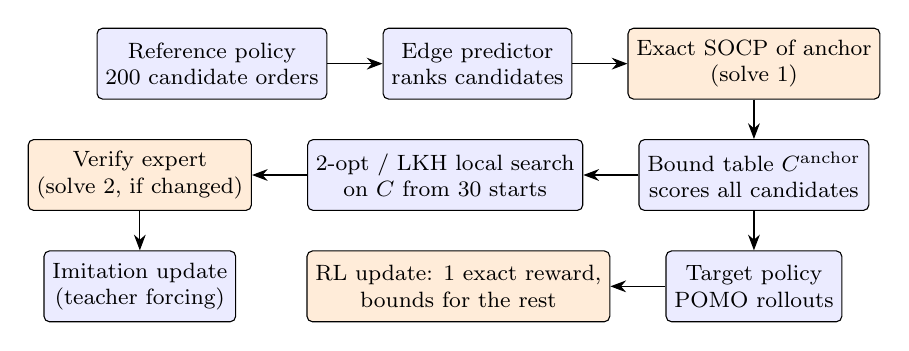
\begin{tikzpicture}[node distance=5mm and 7mm, >={Stealth[length=2mm]},
  box/.style={draw, rounded corners=2pt, align=center, font=\footnotesize, minimum height=9mm, inner sep=3pt},
  exact/.style={box, fill=orange!15}, free/.style={box, fill=blue!8}]
\node[free] (ref) {Reference policy\\200 candidate orders};
\node[free, right=of ref] (pred) {Edge predictor\\ranks candidates};
\node[exact, right=of pred] (anc) {Exact SOCP of anchor\\(solve 1)};
\node[free, below=of anc] (tab) {Bound table $C^{\text{anchor}}$\\scores all candidates};
\node[free, left=of tab] (ls) {2-opt / LKH local search\\on $C$ from 30 starts};
\node[exact, left=of ls] (exp) {Verify expert\\(solve 2, if changed)};
\node[free, below=of exp] (il) {Imitation update\\(teacher forcing)};
\node[free, below=of tab] (tgt) {Target policy\\POMO rollouts};
\node[exact, left=of tgt] (rl) {RL update: 1 exact reward,\\bounds for the rest};
\draw[->] (ref) -- (pred); \draw[->] (pred) -- (anc); \draw[->] (anc) -- (tab);
\draw[->] (tab) -- (ls); \draw[->] (ls) -- (exp); \draw[->] (exp) -- (il);
\draw[->] (tgt) -- (rl); \draw[->] (tab) -- (tgt);
\end{tikzpicture}}
\caption{An illustration of one training step for one instance. Orange boxes call the exact SOCP solver; blue
boxes are solve-free. \todo{redraw as a polished figure.}}\label{fig:framework}
\end{figure}

\subsection{MDP formulation}\label{sec:mdp}

\paragraph{State} The state at step $t$ is $s_t=(x,\pi_{<t})$, where $x$ is the instance and
$\pi_{<t}=(\pi_1,\dots,\pi_{t-1})$ is the partial visiting order. At step 1 the order is empty and the carrier is
at the depot.

\paragraph{Action} An action $a_t$ selects an unvisited target as the next sortie, $\pi_t=a_t$. Visited targets
are masked. In POMO decoding the first action is fixed to one of $P$ distinct start targets.

\paragraph{Transition} The selected target is appended to the partial order, $s_{t+1}=(x,\pi_{<t}\oplus a_t)$.
The episode ends after $n$ steps with a complete order $\pi$.

\paragraph{Reward} After a complete order is constructed, its makespan is obtained by solving the SOCP
\eqref{eq:obj}--\eqref{eq:carrier}, and the reward is $R(\pi)=-f(\pi)$. During training, our method replaces
most exact rewards by certified upper bounds (Section~\ref{sec:training}).

\paragraph{Policy} The probability of a complete order is $p_\theta(\pi\mid x)=\prod_{t=1}^{n}p_\theta(a_t\mid s_t)$.

The take-off and landing points are not part of the MDP. They are continuous, interact across consecutive
sorties, and are optimal only for a complete order, so the policy decides the order and the SOCP decides the
geometry. This division keeps the action space discrete but makes the reward sparse and expensive, which is the
difficulty our training procedure addresses.

\subsection{Policy network}\label{sec:policy}
The policy follows the attention encoder--decoder of \citet{kool2019attention} in its POMO form
\citep{kwon2020pomo}.

\paragraph{Input features} Each node $j\in\{0,\dots,n\}$ (depot and targets) is described by
$v_j=(\tilde p_j,\ \|\tilde p_j\|,\ \mathbb{1}[j=0],\ V_c/V_v,\ V_v a/D)\in\R^6$, where
$\tilde p_j=(p_j-p_0)/D$ is the position relative to the depot normalised by the instance scale $D$. The last two
features are the same for all nodes; they tell the network how far the drone can reach relative to the carrier's
movement, which determines how much the carrier can save by launching early or recovering late.

\paragraph{Encoder} A linear layer maps $v_j$ to $h^{(0)}_j\in\R^{d}$ with $d=256$. Each of $L=4$ encoder layers
applies multi-head self-attention \citep{vaswani2017attention} with 16 heads, a skip connection with instance
normalisation, a feed-forward layer with hidden dimension 512, and a second skip connection with instance
normalisation:
\begin{equation}
\hat h_j=\mathrm{Norm}\big(h^{(l-1)}_j+\mathrm{MHA}_j(h^{(l-1)}_0,\dots,h^{(l-1)}_n)\big),\qquad
h^{(l)}_j=\mathrm{Norm}\big(\hat h_j+\mathrm{FF}(\hat h_j)\big).
\end{equation}

\paragraph{Decoder} At step $t$ the context query combines the embeddings of the first and the last visited
target, $q_t=W_{\mathrm{f}}h^{(L)}_{\pi_1}+W_{\mathrm{l}}h^{(L)}_{\pi_{t-1}}$. A masked multi-head attention over
all node embeddings gives a glimpse $g_t$, and a single-head compatibility gives the probabilities
\begin{equation}
u_{tj}=C\tanh\!\Big(\frac{g_t^{\top}h^{(L)}_j}{\sqrt d}\Big),\qquad
p_\theta(a_t=j\mid s_t)=\frac{\exp(u_{tj})}{\sum_{j'\notin\pi_{<t}}\exp(u_{tj'})}\quad(j\notin\pi_{<t}),
\end{equation}
with clipping constant $C=10$.

\paragraph{Inference} At test time the policy decodes greedily from $\min(n,100)$ start targets on each of
eight geometric views of the instance (rotations and reflections). Every distinct order is solved exactly and
the best makespan is returned. The exact solves at inference are needed to obtain an executable plan and are the
same for all learned models compared in this paper.

\subsection{Certified upper-bound tables}\label{sec:ubtable}
Let $q$ be an order and let $(s^*,l^*,t^{\mathrm{out}*},t^{\mathrm{in}*},\tau^*)$ be an optimal solution of the
SOCP for $q$. Relabel the sortie variables by target: for target $j=q(k)$ write $\hat s_j=s^*_k$,
$\hat l_j=l^*_k$ and $\hat\tau_j=\tau^*_k$. Define the directed table $C^q\in\R^{(n+1)\times(n+1)}$ with
\begin{equation}\label{eq:table}
C^q_{0j}=\frac{\|\hat s_j-p_0\|}{V_c},\qquad
C^q_{ij}=\hat\tau_i+\frac{\|\hat s_j-\hat l_i\|}{V_c},\qquad
C^q_{i0}=\hat\tau_i+\frac{\|p_0-\hat l_i\|}{V_c},
\end{equation}
for $i,j\in\{1,\dots,n\}$, $i\ne j$, and for any order $\pi$ the route sum
$\UB_q(\pi)=C^q_{0\pi(1)}+\sum_{k=1}^{n-1}C^q_{\pi(k)\pi(k+1)}+C^q_{\pi(n)0}$.

\begin{proposition}\label{prop:ub}
For every order $\pi$, $f(\pi)\le \UB_q(\pi)$, and $f(q)=\UB_q(q)$.
\end{proposition}
\begin{proof}
Assign to sortie $k$ of $\pi$ the relabelled values of target $\pi(k)$: $s_k=\hat s_{\pi(k)}$,
$l_k=\hat l_{\pi(k)}$, and the corresponding drone times. Constraints \eqref{eq:end}--\eqref{eq:sync} involve
only the variables of one sortie and its own target, so they hold because they held for $q$. Set
$T_k=\|s_k-l_{k-1}\|/V_c$ and $T_{n+1}=\|p_0-l_n\|/V_c$; then \eqref{eq:carrier} holds with equality. The
solution is feasible for the SOCP of $\pi$ and its objective equals $\UB_q(\pi)$, hence $f(\pi)\le\UB_q(\pi)$.
For $\pi=q$ the carrier legs of an optimal solution are tight, so the objective equals $f(q)$.
\end{proof}

The table is asymmetric, since $\hat s_j\neq\hat l_j$ in general. It is tight at the anchor $q$ and loose for
orders that would move the take-off and landing points far from their anchor positions. A move that changes a
few adjacencies, such as 2-opt, changes $\UB_q$ by a few table entries, so it can be evaluated in constant
time.\footnote{For a directed table a 2-opt move reverses a segment, and all directed edges inside the segment
change; the implementation computes these deltas incrementally with prefix sums.} The minimum of several tables,
$\min_m \UB_{q_m}(\pi)$, is again a certified bound. In contrast, the entry-wise minimum of two tables is not,
because it splices two different primal solutions.

\subsection{Expert search on the bound table}\label{sec:expert}
For each training instance a frozen \emph{reference} policy samples 200 candidate orders. A lightweight directed
edge predictor, trained on the tables of earlier batches with a Huber loss, ranks them and selects the
\emph{anchor} to be solved exactly (solve~1). The anchor's table $C^{\text{anchor}}$ then scores all candidates
in the sense of Proposition~\ref{prop:ub}.

Local search starts from 30 candidates: the 20 with the lowest bound and 10 chosen for diversity from the next 60,
provided their bound is within 5\% of the best. From each start we run first-improvement 2-opt on
$C^{\text{anchor}}$ for at most 30 accepted moves, accepting only a strict decrease of the bound. Because
$\UB_{\text{anchor}}(\text{anchor})=f(\text{anchor})$, any route whose bound is below the anchor's exact makespan
is certified to be strictly better than the anchor. The route with the lowest bound becomes the \emph{expert}. If
it differs from the anchor, it is solved exactly (solve~2), so the expert label always carries its exact makespan,
and its own table $C^{\text{expert}}$ becomes available.

Two mechanisms recover improvements that a single loose table misses. \emph{Near-miss validation}: when no route
certifies an improvement, the best non-anchor route is solved exactly with a probability between 1\% and 5\% that
adapts to the policy's imitation accuracy, and it is accepted if its exact makespan beats the anchor.
\emph{Table refresh}: for large instances later in training (Section~\ref{sec:recipe}), the search is repeated on
the table of the latest solved route, which is tight in a different region of the order space, and the best
unsolved result is solved and accepted only if it is exactly better.

\subsection{Training procedure}\label{sec:training}

\paragraph{Hybrid policy gradient} The trainable \emph{target} policy samples $P$ POMO rollouts
$\pi^{1},\dots,\pi^{P}$ per instance. Their costs are the tighter of the two available bounds,
\begin{equation}\label{eq:hybridcost}
c^{p}=\min\{\UB_{\text{anchor}}(\pi^{p}),\ \UB_{\text{expert}}(\pi^{p})\},\qquad p=1,\dots,P,
\end{equation}
except for one selected rollout whose cost is its exact makespan (solve~3). Advantages are centred by the POMO mean
and standardised within the instance, $A^{p}=-(c^{p}-\bar c)/\max(\sigma_c,\epsilon)$, and the loss for a batch of
$B$ instances is
\begin{equation}\label{eq:lrl}
\mathcal L_{\mathrm{RL}}=-\frac{1}{BP}\sum_{b=1}^{B}\sum_{p=1}^{P}A^{p}_b\log p_\theta(\pi^{p}_b\mid x_b).
\end{equation}
An auxiliary term rewards the exactly solved rollout relative to the exact expert makespan, clipped to $[-1,1]$ in
relative terms; its weight rises from 0 to 1 as the imitation accuracy of the previous epoch grows from 0.50 to
0.85. Since every bound is certified, a rollout can be over-penalised but never credited with a makespan it
cannot achieve.

\paragraph{Imitation of verified experts} The imitation update is a separate optimiser step on the
teacher-forced cross-entropy of verified expert routes $e$,
\begin{equation}\label{eq:lil}
\mathcal L_{\mathrm{IL}}=-\frac{1}{n}\sum_{t=1}^{n}\log p_\theta(e_t\mid x,e_{<t}),
\end{equation}
for five inner passes over a buffer that mixes the current batch with 30\% replayed experts from a buffer of
50{,}000. Experts that improve on the anchor are up-weighted so that the imitation mass per instance stays near a
fixed target (1.44 samples per instance) as the improvement rate changes. At the end of each epoch the reference
policy is replaced by the target policy only if the target is strictly better on a fixed set of validation
instances.

\paragraph{Progressive search schedule}\label{sec:recipe}
Early in training the policy is weak and almost any 2-opt search improves it; later the policy itself proposes
2-opt-optimal routes and the expert stops improving, mostly for large instances. Stronger search everywhere,
however, collapses the diversity of the POMO rollouts for small instances. We therefore strengthen the expert only
for $n\ge60$ and only gradually. With the ramp $r=\mathrm{clip}((\text{epoch}-40)/60,0,1)$, a fraction $0.5\,r$ of
the local-search starts uses LKH-3 \citep{helsgaun2017lkh3} on the bound table instead of 2-opt, the near-miss
probability rises to $\rho+r(1-\rho)$ (100\% from epoch 100), and two table-refresh rounds are run from epoch 61.
Instances with $n<60$ keep plain 2-opt and adaptive near-miss validation throughout.

\paragraph{Exact-solve accounting} Per instance, training uses one solve for the anchor, one for the exactly
rewarded rollout, at most one for the expert or near-miss route, and, for large instances late in training, one
per refresh round. The number of solves does not depend on the number of POMO rollouts or local-search moves. Over
the whole run the average is 2.89 solves per training instance (Table~\ref{tab:budget}), whereas exact-reward
training solves every distinct sampled route. Algorithm~\ref{alg:train} summarises one training step.

\begin{algorithm}[t]
\caption{Self-improving training (one batch $\mathcal B$)}\label{alg:train}
\begin{algorithmic}[1]
\For{each instance $x\in\mathcal B$ \textbf{in parallel}}
  \State sample 200 orders from the reference policy; choose anchor $q$ by the edge predictor
  \State solve the SOCP of $q$ exactly; build $C^{q}$ by \eqref{eq:table} \Comment{solve 1}
  \State score all candidates by $\UB_q$; select 20 best + 10 diverse starts
  \State run 2-opt (or LKH for large $n$) on $C^q$ from each start \Comment{no solves}
  \State $e\gets$ route with lowest bound; \textbf{if} $e\ne q$ \textbf{then} solve $e$ exactly \Comment{solve 2}
  \State \textbf{else} with probability $\rho$ solve the best non-anchor route (near miss)
  \State optional table refresh rounds (large $n$, later epochs)
\EndFor
\State roll out $P$ POMO routes per instance with the target policy; solve one exactly \Comment{solve 3}
\State RL step on \eqref{eq:lrl} with costs \eqref{eq:hybridcost}; IL step on \eqref{eq:lil} with replay
\State update the edge predictor on the new tables
\State \textbf{at epoch end:} replace reference by target if strictly better on fixed validation instances
\end{algorithmic}
\end{algorithm}

%% ===================================================================
\section{Experiments}\label{sec:exp}

We evaluate the method on synthetic and benchmark instances against a policy trained with exact rewards, an exact
MISOCP solver and metaheuristics. The training cost is compared in detail, the effects of methodological
components are verified by an ablation study, and generalisation to larger instances is tested.

\subsection{Experimental setup}\label{sec:setup}
Following the synthetic data generation in DRL research \citep{kool2019attention,kwon2020pomo}, we place the depot
and $n$ targets uniformly in the unit square, with $V_c=0.2$, $V_v\sim U[0.4,1.0]$ (speed ratio 2--5) and
$a\sim U[0.05,1.0]$; these are the normalised parameter ranges of the benchmark instances. Training samples $n$
uniformly from $\{20,\dots,100\}$ and generates 10{,}000 fresh instances per epoch, with batch size 64 and Adam
with learning rate $10^{-4}$ decaying by cosine to $10^{-7}$. Models are selected on a validation set of 2{,}000
instances (400 for each $n\in\{20,40,60,80,100\}$) and tested once on a test set of 500 instances (100 per size)
that is never used for any decision. Generalisation sets contain 100 instances each with
$n\in\{150,200,300,500\}$. Our final model (\textbf{Ours}) is the checkpoint of epoch 133, selected on the
validation set among all epochs of a 200-epoch run. Experiments run on one Intel i9-13900KF (32 threads) with one
NVIDIA RTX 4090; Gurobi uses one thread per solve.

The benchmark set (\emph{Real529}) consists of the 72 instances of \citet{gambella2018exact} (Gam72, $n=10$--15),
the 132 of \citet{erdogan2021exact} (Erd132, $n=16$--50) and the 325 of \citet{poikonen2020mothership} (Poi325,
regular and clustered layouts, $n=10$--200), as compiled by \citet{li2025exact}. The best-known solution (BKS) of
an instance is the best upper bound reported by any method in the per-instance results of \citet{li2025exact};
optimality is proven for 131 of the 132 instances with $n\le20$ in Gam72 and Erd132 and for 56 instances of Poi325.

We compare with the following methods. \textbf{G200} is POMO with the same architecture trained for 200 epochs of
100{,}000 instances with the exact SOCP makespan as the reward of every rollout; it is the strongest learned
reference. \textbf{POMO-eq} is the same algorithm stopped when its number of exact solves equals that of our
final model. \textbf{MISOCP} is the Model+ formulation of \citet{li2025exact} solved by Gurobi with one thread
and a 3{,}600\,s limit. \textbf{ILS}, \textbf{VNS} and \textbf{SA} are iterated local search, variable neighbourhood
search and simulated annealing over visiting orders; they use the same exact SOCP evaluator with a cache, start
from a nearest-neighbour route improved by Euclidean 2-opt, and use granular neighbourhoods of the eight nearest
targets \citep{toth2003granular}. Their time budgets are 1, 3 and 10 times our single-core inference time per
instance. All learned models use the inference protocol of Section~\ref{sec:policy}. The gap of a method on an
instance is computed relative to the best objective value found among the compared methods (synthetic sets) or to
the BKS (Real529); paired differences are reported with 95\% bootstrap confidence intervals.

\subsection{Comparative results}\label{sec:synthetic}
%% Source: outputs/pomo_gurobi_equal_budget_20261027/eval_equal_solves_test500_aug8/results.json
%% Gap: mean per-instance gap to the best of G200 / Ours / POMO-eq (computed 2026-11-02).
Table~\ref{tab:test500} reports the results on the test set. G200 attains the best objective values for every
size, at the price of 78 times more exact solves in training (Section~\ref{sec:efficiency}). Our approach is
1.05\% above G200 in mean makespan (95\% CI [0.93, 1.18]), from 0.39\% at $n=20$ to about 1.3\% at $n=80$--100.
Under the same solve budget, exact-reward training is much weaker: POMO-eq is 4.21\% worse than our approach
overall (95\% CI [3.76, 4.68]) and 8.35\% worse at $n=100$. The advantage of sparse feedback therefore grows
with the instance size, which is exactly where exact rewards are most expensive. \todo{fill MISOCP, ILS and VNS
rows on test500 and the inference times.}

\begin{table}[t]\centering\small
\caption{Results on the synthetic test set (100 instances per size). Obj.: mean makespan; Gap: mean gap to the
best method on each instance (\%); Time: mean wall time per instance.}\label{tab:test500}
\resizebox{\textwidth}{!}{%
\begin{tabular}{l rrr rrr rrr rrr rrr}
\toprule
\multirow{2}{*}{Method} & \multicolumn{3}{c}{$n=20$} & \multicolumn{3}{c}{$n=40$} & \multicolumn{3}{c}{$n=60$}
 & \multicolumn{3}{c}{$n=80$} & \multicolumn{3}{c}{$n=100$} \\
\cmidrule(lr){2-4}\cmidrule(lr){5-7}\cmidrule(lr){8-10}\cmidrule(lr){11-13}\cmidrule(lr){14-16}
 & Obj. & Gap & Time & Obj. & Gap & Time & Obj. & Gap & Time & Obj. & Gap & Time & Obj. & Gap & Time \\
\midrule
MISOCP (3600\,s) & \todo{} & & & & & & & & & & & & & & \\
ILS ($10\times$) & \todo{} & & & & & & & & & & & & & & \\
VNS ($10\times$) & \todo{} & & & & & & & & & & & & & & \\
\midrule
POMO-eq & 12.489 & 0.63 & \todo{} & 15.849 & 2.20 & & 18.626 & 4.38 & & 20.487 & 6.16 & & 23.211 & 9.22 & \\
G200    & \textbf{12.416} & \textbf{0.03} & & \textbf{15.500} & \textbf{0.10} & & \textbf{17.782} & \textbf{0.08} &
 & \textbf{19.242} & \textbf{0.14} & & \textbf{21.154} & \textbf{0.09} & \\
Ours    & 12.464 & 0.48 & & 15.634 & 1.12 & & 17.988 & 1.39 & & 19.491 & 1.62 & & 21.422 & 1.48 & \\
\bottomrule
\end{tabular}}
\end{table}

\subsection{Training efficiency}\label{sec:efficiency}
%% Source: outputs/bks_comparison_20261023/advantage_table.md
Table~\ref{tab:budget} compares the training cost of G200 and our approach. Our approach sees 15 times fewer
instances and makes 78 times fewer exact solves; measured solver CPU time is about 30 times lower. The wall time
is about 11 times shorter with a quarter of the solver workers, although the two runs used different machines.
Inference is identical because the architecture and test protocol are the same. Fig.~\ref{fig:efficiency} plots
validation quality against the cumulative number of exact solves and of training instances. At every budget our
approach is ahead of exact-reward POMO training from scratch, and it reaches a given validation makespan with one
to two orders of magnitude fewer solves. \todo{24-hour training curves: validation makespan against wall time for
POMO with exact rewards and for our approach; G200 as a horizontal reference.}

\begin{table}[t]\centering\small
\caption{Training budget of POMO with exact rewards (G200) and our approach.}
\label{tab:budget}
\resizebox{\textwidth}{!}{%
\begin{tabular}{lrrr}
\toprule
 & G200 & Ours & Ratio \\
\midrule
Training epochs & 200 & 133 & \\
Training instances & 20{,}000{,}000 & 1{,}330{,}000 & $15\times$ fewer \\
Exact SOCP solves in training & 299{,}437{,}760 & 3{,}839{,}970 & $78\times$ fewer \\
Exact solves per training instance & 15.0 & 2.89 & \\
Solver CPU time (core-h) & $\approx$2{,}580$^{a}$ & 86.7 & $\approx30\times$ less \\
Training wall time (h) & $\approx$215.5$^{b}$ & 19.2 & $\approx11\times$ shorter \\
Solver workers & 128 & 32 & \\
Inference time per instance (s, wall / single-core) & 0.78 / 10.3 & 0.78 / 10.3 & same \\
\bottomrule
\end{tabular}}
\par\smallskip\raggedright\footnotesize
$^{a}$ Estimated as solves $\times$ 0.031\,s, the measured mean SOCP time at $n\approx60$.
$^{b}$ 64.7\,min per epoch measured over epochs 184--188 on a different machine, times 200 epochs.
\todo{replace the estimates by the measured values of the from-scratch run.}
\end{table}

\begin{figure}[t]\centering
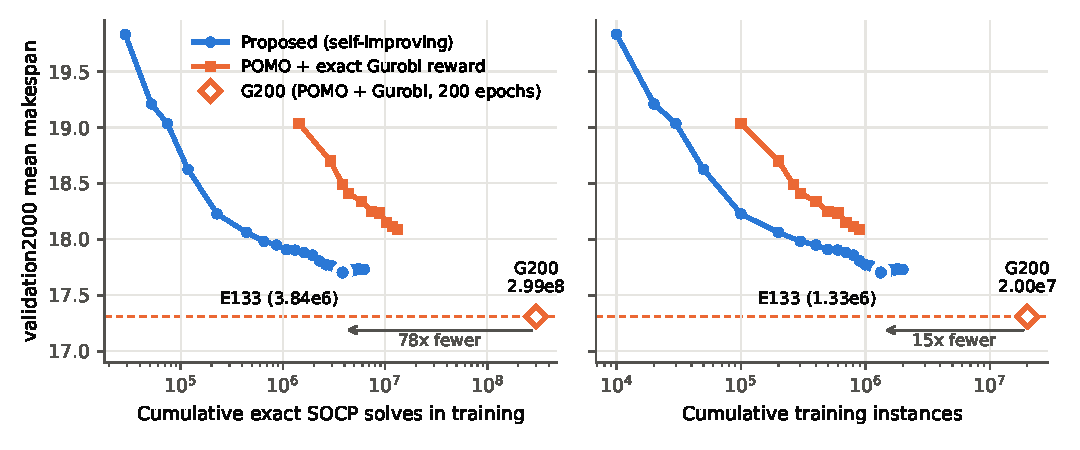
\includegraphics[width=\textwidth]{figures/data_efficiency.pdf}
\caption{Validation mean makespan (full POMO, no augmentation) against cumulative exact SOCP solves (left) and
training instances (right), both on log scales. POMO with exact Gurobi rewards is trained from scratch with the
G200 recipe; G200 is its 200-epoch model.}\label{fig:efficiency}
\end{figure}

\subsection{Ablation study}\label{sec:ablation}
To verify the effects of the components of our approach, we train four variants from scratch with the same
instance stream and compare them at 1{,}000{,}000 training instances (epoch 100) on the validation and test sets.
(A) POMO with exact rewards on every rollout, i.e.\ no sparse feedback. (B) No certified bound table: the expert
search evaluates every candidate route by an exact SOCP solve, which forces a much smaller search (one start,
first-improvement 2-opt in random move order, at most 100 exact solves per instance). (C) The full approach.
(D) No diversity: the expert search starts from a single route, the greedy route of the reference policy, with the
same total search effort as the 30 starts of (C). Variant (B) isolates the value of the bound table: whether a
search restricted to exact evaluation can produce experts of similar quality, and at what training time.
\todo{results; bar chart of objective, gap and training time as in the reference paper, Fig.~3.}

\begin{table}[t]\centering\small
\caption{Ablation results at epoch 100: mean makespan, training wall time and exact solves.
\todo{fill in when the runs finish.}}\label{tab:ablation}
\resizebox{\textwidth}{!}{%
\begin{tabular}{llrrrr}
\toprule
 & Variant & Validation & Test & Wall time (h) & Exact solves \\
\midrule
A & POMO with exact rewards & \todo{} & \todo{} & \todo{} & \todo{} \\
B & w/o bound table (exact search, $\le100$ solves) & \todo{} & \todo{} & \todo{} & \todo{} \\
C & full approach (epoch 100) & \todo{} & \todo{} & $\approx$11 & \todo{} \\
D & w/o diversity (single start) & \todo{} & \todo{} & \todo{} & \todo{} \\
\bottomrule
\end{tabular}}
\end{table}

\subsection{Benchmarking results}\label{sec:real529}
%% Sources: outputs/bks_comparison_20261023 (BKS = best of all methods in Li et al. 2025);
%% outputs/pomo_gurobi_equal_budget_20261027/eval_equal_solves_real529;
%% outputs/metaheuristics_real529_20261026/summary.md (time budgets);
%% outputs/full_gurobi_20261030/real529_3600s (128 of 529 instances, run paused 2026-10-30).
We evaluate all methods on Real529 with the policies trained on synthetic instances. Table~\ref{tab:real529}
reports the gap to the BKS by instance set; Table~\ref{tab:real529size} in \ref{app:detail} gives every size. Both
learned policies are within 0.2\% of the BKS on Gam72 and within 0.6\% on Erd132, where the BKS is mostly optimal,
and find new best solutions on Poi325, where the BKS comes from heuristics (G200: 10 instances; ours: 5). Overall
our approach is 0.12\% above G200 in mean makespan (95\% CI [0.004, 0.229]); on the 25 instances with $n=200$,
outside the training range, it is 1.26\% \emph{better}. POMO-eq is 4.60\% from the BKS, against 1.35\% for our
approach. Both learned policies need 0.78\,s of wall time per instance on average.

At equal time, the metaheuristics are 2.9--4.5\% from the BKS; ILS and VNS need about ten times our single-core
time to overtake our approach, and then mainly on the clustered Poi325 instances. On Erd132 with $n=25$--50 our
approach remains better even at ten times the time. The exact MISOCP is not competitive beyond small instances.
So far it has been run on the 128 largest instances: on all 50 instances with $n=100$ and all 25 with $n=200$ Gurobi
found \emph{no feasible solution} within one hour, and on the 53 instances with $n=50$ the final MIP gap averaged
39\% and the incumbent was on average 23\% worse than our approach, which needs 0.8--5.6\,s for these instances.
\todo{complete the MISOCP run and add it as a column of Table~\ref{tab:real529}.}
\todo{verify SA: its $1\times$ and $3\times$ results coincide and Erd132 $n=25$--50 stays at 5.57\% for every
budget.}

\begin{table}[t]\centering\small
\caption{Results on Real529: mean gap to the BKS (\%) by instance set. Metaheuristic budgets are multiples of our
single-core inference time per instance (10.3\,s on average). W/T/L: instances where the method is better / equal
/ worse than ours.}
\label{tab:real529}
\resizebox{\textwidth}{!}{%
\begin{tabular}{llrrrrrrr}
\toprule
Method & Budget & Gam72 & Erd 16--20 & Erd 25--50 & Poi Regular & Poi Cluster & All & W/T/L vs ours \\
\midrule
ILS & $1\times$  & 1.20 & 1.40 & 4.21 & 5.03 & 1.30 & 2.93 & 175/83/271 \\
ILS & $3\times$  & 0.71 & 0.80 & 3.08 & 2.79 & 0.36 & 1.63 & 251/98/180 \\
ILS & $10\times$ & 0.33 & 0.27 & 1.90 & \textbf{1.22} & $-0.02$ & \textbf{0.73} & 321/116/92 \\
VNS & $1\times$  & 1.20 & 1.40 & 4.21 & 5.04 & 1.31 & 2.93 & 175/83/271 \\
VNS & $3\times$  & 0.69 & 0.76 & 3.14 & 2.84 & 0.36 & 1.65 & 251/100/178 \\
VNS & $10\times$ & 0.20 & 0.34 & 1.89 & 1.40 & $\mathbf{-0.03}$ & 0.78 & 314/120/95 \\
SA  & $1\times$  & 1.65 & 2.13 & 5.57 & 7.48 & 2.93 & 4.53 & 63/73/393 \\
SA  & $10\times$ & 0.53 & 1.27 & 5.15 & 5.16 & 1.84 & 3.14 & 154/100/275 \\
\midrule
POMO-eq & -- & 0.61 & 1.54 & 6.28 & 6.41 & 4.82 & 4.60 & \\
G200 & -- & \textbf{0.01} & \textbf{0.08} & \textbf{0.80} & 1.59 & 1.76 & 1.14 & 246/159/124 \\
Ours & -- & 0.19 & 0.24 & 0.89 & 1.75 & 2.10 & 1.35 & -- \\
\bottomrule
\end{tabular}}
\end{table}

\subsection{Generalisation to larger instances}\label{sec:generalisation}
%% Source: outputs/generalization_20261029/eval_aug8/results.json
Both policies were trained with $n\le100$. Table~\ref{tab:general} tests them on $n=150$--500. The gap of our
approach to G200 shrinks from about 1.3\% at $n=80$--100 to 0.81\% at $n=150$, 0.73\% at $n=200$, 0.19\% (not
significant) at $n=300$ and 0.48\% at $n=500$. This suggests that the bound-guided experts teach a construction
rule that transfers to larger instances at least as well as one learned from exact rewards.

\begin{table}[t]\centering\small
\caption{Generalisation results: mean makespan (8 views) on 100 instances per size, relative difference of ours
to G200 (95\% bootstrap CI), and our wins/ties/losses against G200.}\label{tab:general}
\begin{tabular}{rrrrr}
\toprule
$n$ & G200 & Ours & Ours vs G200 (\%) & W/T/L \\
\midrule
150 & 25.795 & 26.003 & $+0.81$ [0.46, 1.17] & 23/0/77 \\
200 & 28.868 & 29.077 & $+0.73$ [0.31, 1.14] & 30/0/70 \\
300 & 36.875 & 36.945 & $+0.19$ [$-0.20$, 0.60] & 42/0/58 \\
500 & 51.040 & 51.283 & $+0.48$ [0.15, 0.80] & 40/0/60 \\
\midrule
All & 35.644 & 35.827 & $+0.51$ [0.33, 0.70] & 135/0/265 \\
\bottomrule
\end{tabular}
\end{table}

%% ===================================================================
\section{Conclusion}\label{sec:conc}
We presented a self-improving DRL approach to the carrier--vehicle traveling salesman problem that learns from
sparse exact feedback. Its key element is a certified upper-bound table built from one exact SOCP solution, which
scores any visiting order and supports fast local search without further solves. Combined with imitation of
verified expert routes and policy gradients on hybrid exact/bound rewards, the approach trains a policy close to
one trained on exact rewards for every rollout, with 78 times fewer exact solves and the same inference cost. Under
an equal solve budget it clearly outperforms exact-reward training, and it generalises to instances with up to 500
targets. For practice, this turns retraining for a new vessel speed, drone model or service region from a
nine-day job on a solver cluster into an overnight job on one workstation, and the trained policy plans a
100-target mission in seconds, fast enough for replanning during the mission.
The policy remains about 1\% behind G200 on synthetic instances with 40--100 targets; our analysis suggests that
the self-improving updates reduce the diversity of the POMO rollouts, which matters when the best of many rollouts
is returned. In the future, we will study how to preserve this diversity, and extend the idea of sharing one exact
solution across many routes to other routing problems whose route cost is the value of a convex program, such as
truck--drone problems with continuous rendezvous or routing with speed optimisation.

\section*{CRediT authorship contribution statement}
\todo{}

\section*{Data availability}
\todo{code and instances repository}

\section*{Declaration of competing interest}
The authors declare that they have no known competing financial interests or personal relationships that could
have appeared to influence the work reported in this paper.

\section*{Acknowledgement}
\todo{funding}

\appendix
\section{Detailed Real529 results by instance size}\label{app:detail}
%% Source: outputs/bks_comparison_20261023/timing/{epoch200,new_e133}.json with best_known_all_methods.json
\begin{table}[p]\centering\footnotesize
\caption{Real529 by set and size $n$ (number of instances in parentheses). UB: mean makespan; $\Delta$: mean gap
to BKS (\%); BS/NBS: instances reaching / improving the BKS; Time: our mean wall seconds per instance (G200's is
the same within 0.02\,s).}\label{tab:real529size}
\resizebox{\textwidth}{!}{%
\begin{tabular}{lr r rrr rrr r}
\toprule
 & & & \multicolumn{3}{c}{G200} & \multicolumn{3}{c}{Ours} & \\
\cmidrule(lr){4-6}\cmidrule(lr){7-9}
Set & $n$ (\#) & BKS & UB & $\Delta$ & BS/NBS & UB & $\Delta$ & BS/NBS & Time \\
\midrule
Gam72 & 10 (12) & 210.39 & 210.39 & 0.00 & 12/0 & 211.85 & 0.59 & 8/0 & 0.07 \\
      & 11 (12) & 215.13 & 215.13 & 0.00 & 12/0 & 215.14 & 0.00 & 11/0 & 0.07 \\
      & 12 (12) & 208.99 & 209.00 & 0.01 & 11/0 & 209.14 & 0.10 & 10/0 & 0.08 \\
      & 13 (12) & 221.58 & 221.57 & 0.00 & 12/0 & 221.74 & 0.05 & 11/0 & 0.10 \\
      & 14 (12) & 222.36 & 222.36 & 0.00 & 12/0 & 222.95 & 0.28 & 7/0 & 0.10 \\
      & 15 (12) & 249.38 & 249.43 & 0.02 & 10/0 & 249.68 & 0.08 & 10/0 & 0.12 \\
\midrule
Erd132 & 16 (12) & 332.61 & 332.81 & 0.06 & 10/0 & 334.12 & 0.42 & 7/0 & 0.12 \\
       & 17 (12) & 335.09 & 335.09 & 0.00 & 12/0 & 335.79 & 0.21 & 8/0 & 0.14 \\
       & 18 (12) & 347.56 & 347.63 & 0.02 & 9/0 & 348.06 & 0.14 & 8/0 & 0.14 \\
       & 19 (12) & 346.38 & 346.91 & 0.15 & 8/0 & 346.93 & 0.16 & 7/0 & 0.17 \\
       & 20 (12) & 366.48 & 367.12 & 0.17 & 7/0 & 367.47 & 0.28 & 9/0 & 0.17 \\
       & 25 (12) & 385.31 & 387.28 & 0.49 & 5/0 & 388.13 & 0.71 & 3/0 & 0.25 \\
       & 30 (12) & 407.58 & 408.89 & 0.31 & 4/0 & 409.97 & 0.58 & 4/0 & 0.33 \\
       & 35 (12) & 424.04 & 426.50 & 0.54 & 3/0 & 428.36 & 0.97 & 1/0 & 0.44 \\
       & 40 (12) & 457.04 & 461.35 & 0.93 & 0/0 & 462.64 & 1.19 & 1/0 & 0.54 \\
       & 45 (12) & 483.21 & 489.32 & 1.24 & 4/0 & 485.98 & 0.55 & 4/0 & 0.66 \\
       & 50 (12) & 483.82 & 490.31 & 1.31 & 1/0 & 490.33 & 1.33 & 0/0 & 0.81 \\
\midrule
Poi325 Regular & 10 (25) & 213.74 & 213.78 & 0.02 & 22/1 & 214.15 & 0.19 & 19/1 & 0.07 \\
               & 15 (25) & 240.74 & 241.12 & 0.16 & 12/1 & 242.13 & 0.56 & 8/1 & 0.12 \\
               & 20 (25) & 260.37 & 261.54 & 0.45 & 4/0 & 262.47 & 0.82 & 1/0 & 0.18 \\
               & 30 (25) & 290.64 & 292.09 & 0.50 & 6/1 & 293.15 & 0.84 & 4/0 & 0.34 \\
               & 50 (25) & 355.33 & 358.19 & 0.79 & 3/3 & 361.12 & 1.59 & 1/1 & 0.80 \\
               & 100 (25) & 492.22 & 502.80 & 2.09 & 3/3 & 504.08 & 2.33 & 2/2 & 2.80 \\
               & 200 (25) & 678.28 & 730.12 & 7.09 & 0/0 & 720.93 & 5.91 & 0/0 & 5.56 \\
\midrule
Poi325 Cluster & 10 (25) & 242.11 & 243.10 & 0.40 & 4/0 & 243.34 & 0.49 & 5/0 & 0.08 \\
               & 15 (25) & 252.97 & 255.40 & 0.95 & 0/0 & 255.62 & 1.03 & 0/0 & 0.13 \\
               & 20 (25) & 260.34 & 262.54 & 0.84 & 0/0 & 263.67 & 1.26 & 0/0 & 0.19 \\
               & 30 (25) & 271.54 & 273.82 & 0.83 & 0/0 & 274.65 & 1.13 & 0/0 & 0.36 \\
               & 50 (25) & 292.03 & 296.72 & 1.57 & 1/1 & 298.16 & 2.04 & 0/0 & 0.83 \\
               & 100 (25) & 335.35 & 356.65 & 5.95 & 0/0 & 359.42 & 6.67 & 0/0 & 2.87 \\
\bottomrule
\end{tabular}}
\end{table}

\bibliographystyle{elsarticle-harv}
\bibliography{refs}

\end{document}
